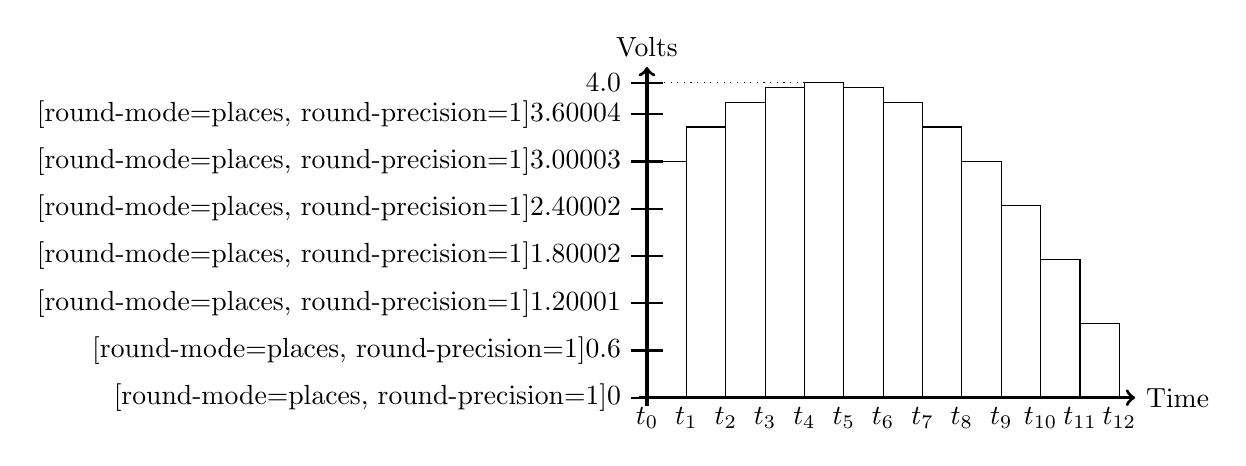
\begin{tikzpicture}[domain=0:6]
    %\draw[very thin,color=gray] (-0.1,-1.1) grid (8*pi, 1.1);
    \draw[->, very thick] (-0.1,0) -- (6.2,0) node[right] {Time};
    \draw[->, very thick] (0,-.1) -- (0,4.2) node[above] {Volts};
    %\draw[color=blue] plot[id=sin,samples=1000] function{-((x-2)*(x-2))+4};
    \draw[color=blue, thick] plot[id=sin,samples=1000] function{-((x/2-1)**2)+4};

	\foreach \x in {0, 0.5, ..., 5.5}
	{
		\draw (\x,0) -- ++(0, {-((\x/2)*(\x/2) - 2*(\x/2)) + 3}) -| ({\x+.5}, 0);
	}

	\foreach \x in {0, ..., 12}
	{
		\draw ({\x/2}, 0) node[below] {$t_{\x}$};
	}

	\foreach \y in {0, 0.6, ..., 4}
	{
		\draw[thick] (.2, \y) -- (-.2, \y) node[left] {\num[round-mode=places, round-precision=1]{\y}};
	}
	\draw[thick] (.2, 4) -- (-.2, 4) node[left] {4.0};
	\draw[dotted] (2, 4) -- (0, 4);



	% vertical axis values

	% tics
\end{tikzpicture}
